\chapter{Introduction} \label{chap_introduction}

Sinds the early days there have been challenges with creating and maintaining stable and
evolvable software. On the one hand, this is caused by constantly evolving requirements as
new business opportunities, technologies, methodologies, and best practices are developed
to meet the demands of modern corporate environments. On the other hand, changing software
can lead to deterioration in stability and evolvability, which can negatively impact the
quality of these systems. \textcite{lehman_programs_1980} has described this as one of his
laws of software evolution: The balance between the forces driving new requirements and
those that slow down progress. These challenges have been recognized by the following
pioneers in software engineering. 

\textcite{d_mcilroy_nato_1968} proposed a vision where the systematic reuse of software
building blocks should lead to more reuse. \textcite{d_mcilroy_nato_1968} quoted
\enquote{The real hero of programming is the one who writes negative code}, i.e. when a
change in a program source makes the number of lines of code decrease ('negative' code),
while its overall quality, readability or speed improves
\footnote{\url{https://en.wikipedia.org/wiki/Douglas_McIlroy}}. Perhaps very early concepts
of modular software constructs?

\textcite{dijkstra_letters_1968} argued against using unstructured control flow in
programming and advocated for using structured programming constructs to improve the
clarity and maintainability of the source code. He advocated structured programming
techniques that improved the modularity and evolvability of software artifacts.

\textcite{parnas_criteria_1972} continued with the principle of information hiding. He
stated that design decisions used multiple times by a software artifact should be
modularized to reduce complexity. 

Various programming paradigms, including procedural, object-oriented, and functional
programming, have emerged to enhance software programming capabilities that contribute to
stability and evolvability \parencite{mannaert_normalized_2016}. These paradigms have
impacted modern programming languages, such as Java and C\#, enabling the development of
more modular and evolvable software architectures.

Design principles, patterns, and theorems are, on top of all, additional measures to
enhance the modularity, stability, and evolvability of software artifacts. As a junior
software engineer, I was always intrigued by the concepts of quality and maintainable code
and quickly got introduced to the \gls{solid} principles. And later on with the complete
design approach derived from Clean Architecture. Starting my Master's degree, I got an
inspiring introduction from Jan Verelst and realized quality and maintainability were
essentially all about the concepts of stability and evolvability. For me, it was very
interesting that the \gls{ns} Theory is supported by empirical scientific evidence.
Although I'm not that active anymore in the field of software engineering, I immediately
knew the topic of my research. it is still a big passion of mine.

Given my experience with Clean Architecture, and what I was learning from Normalized
Systems Theory, I noticed a lot of similarities, but also some big differences. In early
investigations, I found overlapping characteristics. But it seemed there were also a couple
of differences. I wanted to know if the design approaches could be used in conjunction with
each other, perhaps bettering the result of stable and evolvable software.

Java SE has primarily been used for case studies in order to develop the Normalized
Systems Theory \parencite{oorts_building_2014, de_bruyn_enabling_2018}. Although
sufficient in Java, I was pleased to read that both software design approaches have
formulated their modular structures independent of any programming technology
\parencite{mannaert_normalized_2009,robert_c_martin_clean_2018}. So I was free to use my
favorite programming language C\# to create a software artifact that supported my
research, igniting my passion for programming again. 

Based on my early investigations of both design approaches I hypothesized that they can be
used in conjunction with each other. Consequently, an artifact that is designed based on
the principles of Clean Architecture will lead to a highly modular, stable, and evolvable
C\# artifact that does not contradict a design based on the Normalized Systems theorems.

\begin{figure}[H]
    \centering
    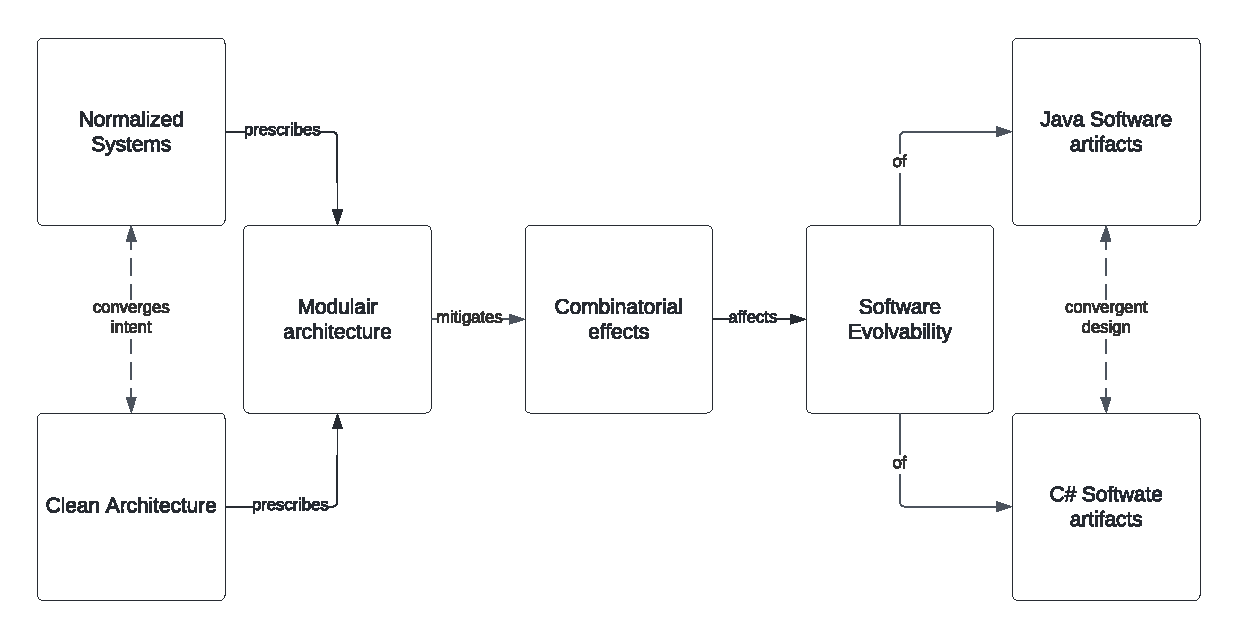
\includegraphics[width=0.8\textwidth]{Figures/hypothesis.pdf}
    \caption[The hypothesis]{The hypothesis}
    \label{fig_hypothesis}
\end{figure}

\section{Research Objectives} \label{sec_research_objectives}

In this Design Science Research, we will shift the focus from Research Questions to
Research Objects. The Object of this research is to determine the degree of convergence of
Clean Architecture, with the Normalized Systems Theory. 

To summarize, we will start with a generic design that is based on the principles and
design characteristics of Clean Architecture. Given this design, we will conduct the
research on two different artifacts, namely a code-generator artifact and a generated
artifact. The reason for the code-generator artifact is to provide strict and meticulous
adherence to the generic design. Each entity should be implemented in exactly the same way.

AFMAKEN



% In this Design Science research, the focus shifts from a research question toward
% research objectives. The following objectives apply to this research.

% \subsection*{Objective 1: The expander artifact}
% A C\# artifact that consists of a source code expander and some helper classes to
% generate the second \emph{expanded} artifact. The artifact supports the harvesting and
% rejuvenation of custom code snippets on the expanded artifact so that regenerations do not
% have a loss of implementations on the expanded artifact. The expander artifact is entirely
% based on the design principles of \gls{ca}.

% Chapter \ref{sec_generator_artifact} entirely describes the expander artifact.

% \subsection*{Objective 2: The expanded artifact}
% This artifact is an entirely working restful API, that is based on ASP.NET and C\#. It has
% essential CRUD support. The artifact has been generated by the \emph{expander} and has
% been enriched with custom code snippets to comply with the initial requirements.
% The expanded artifact is entirely based on the design principles of \gls{ca}.

% Chapter \ref{sec_generator_artifact} entirely describes the expander artifact.


%\section{Research questions} \label{research_questions}
The Hypothesis described in \ref{hypothesis} and \ref{conceptualframework} leads us to the
following research question:

\begin{center}
    \enquote*{\textit{To what extent converges the evolvability of a C\# artifact built
    based on the Clean Architecture principles towards a similar artifact that is based on
    Normalized Systems Theorems?}}
\end{center}

The following sub-questions can be formulated that support the research on the main
research question:
\begin{itemize}
    \item How does Clean Architecture contribute to Software Evolvability?
    \item To what extent Is Normalized Systems applicable to a C\# artifact?   
\end{itemize}
\section{Research method} \label{sec_research_method}

This research is a Design Science Method and relies on the Engineering Cycles as described
by \textcite{wieringa_design_2014}. The engineering cycle provides a structured approach
to develop the required artifacts to analyze the design problem (HIER CITE NAAR WIERINGA).

\begin{figure}[H]
    \centering
    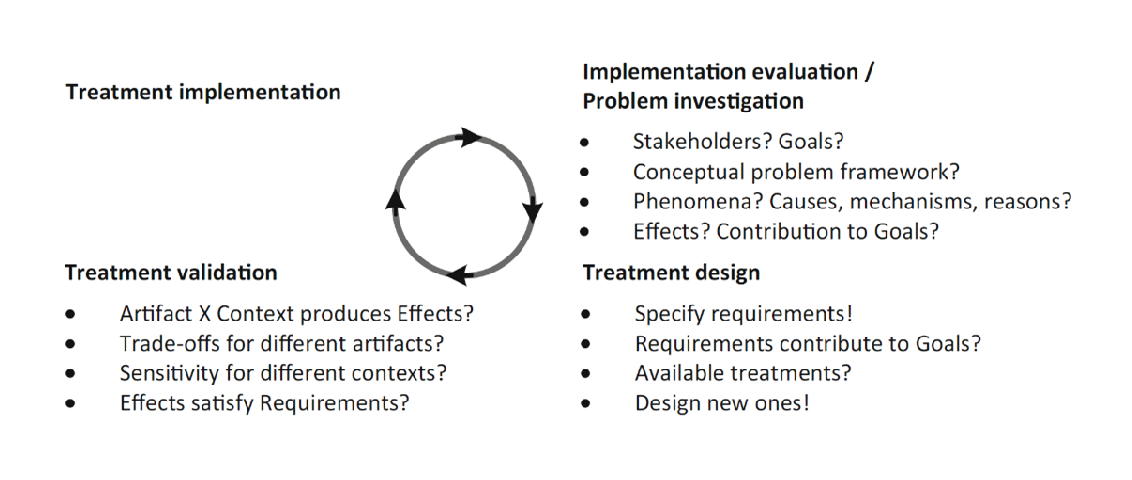
\includegraphics[width=1\textwidth]{Figures/engineering_cycle.pdf}
    \caption[Engineering cycle]{Wieringa's engineering cycle}
    \label{fig_engineering_cycle}
\end{figure}

In the context of this research, the artifacts described in chapters
\ref{sec_generator_artifact} and \ref{sec_generated_artifact} are considered to be
information systems. \citeauthor{hevner_design_nodate} proposed a framework for research
in information systems by introducing the interacting relevance and rigor cycles.

Figure \ref{fig_dsr} depicts a specialized overview of Hevners Design Science Framework.
The rigor cycle is composed of the theories and knowledge from \gls{ns}
and \gls{ca}. This is supplemented by the rigorous knowledge of modularity,
evolvability, and stability of software systems. The Relevance cycle represents the
business needs of the stakeholders. The business needs are described as research
objectives, research questions, and research requirements.

\begin{figure}[H]
    \centering
    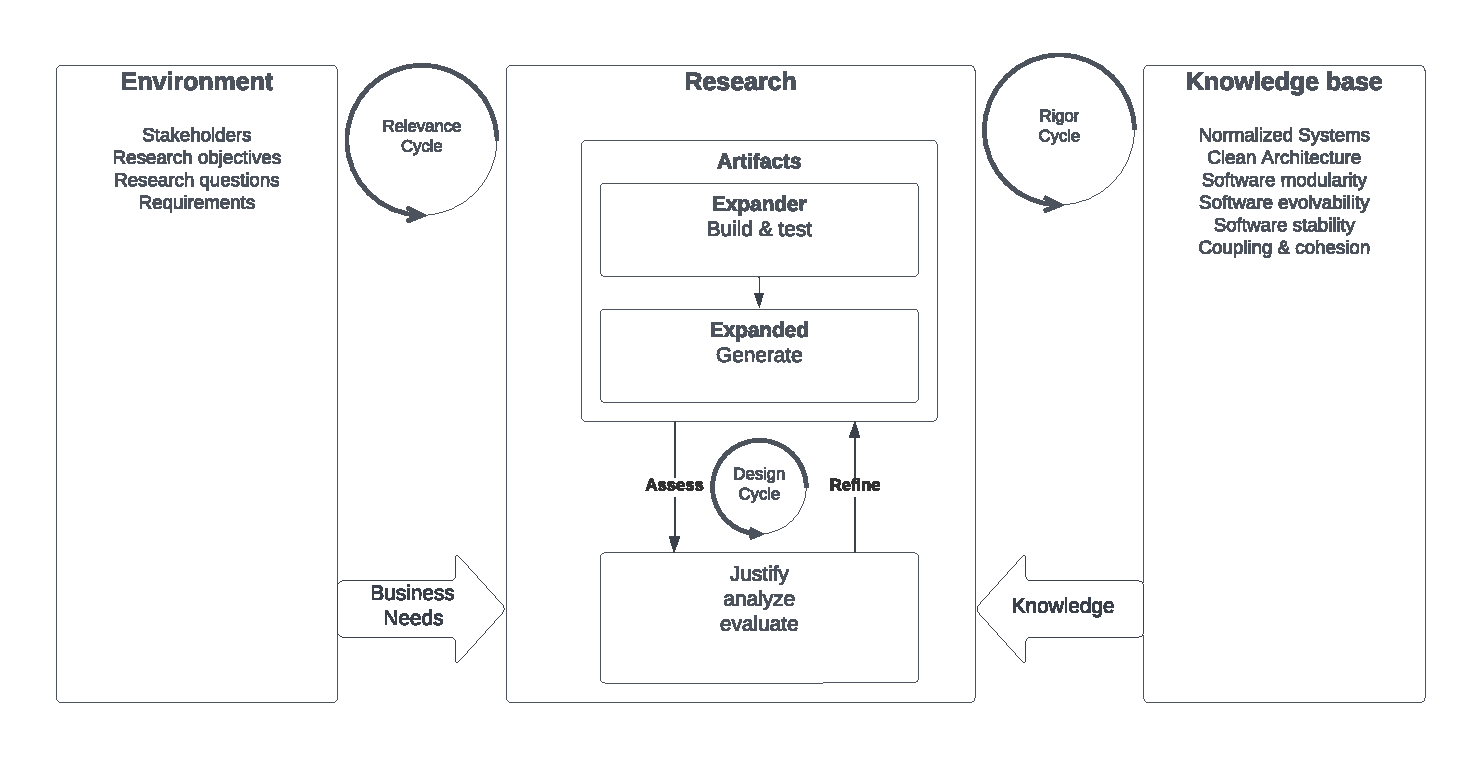
\includegraphics[width=1\textwidth]{Figures/rigor_relevance_cycle.pdf}
    \caption[DSF]{The Design Science Framework for IS Research}
    \label{fig_dsr}
\end{figure}
\section{Thesis outline} \label{sec_structure}

The structure of this thesis reflects the research methodology described in the previous
section \ref{sec_research_method}. Chapter \ref{chap_theoreticalbackground} presents the
theoretical backgrounds of both \ns and \ca, discussing important
characteristics and requirements of software stability, as well as the principles and
architectures proposed by both development approaches.

Chapter \ref{chap_requirements} focuses on the requirements relevant to this research. It
is divided into two sections: section \ref{sec_research_requirements} outlines the
research requirements, describing the requirements necessary for conducting the research,
while section \ref{sec_artifact_requirements} details the artifact requirements, laying
out the requirements relevant to the artifacts contributing to this research.

Chapter \ref{chap_evaluation} evaluates the research results, discussing the impact of
using CA on NS. Notable experiences and findings in Chapter \fullref{chap_discussion}. The
conclusion of this research is presented in the final chapter, Chapter \ref{chap_conclusions}.

Lastly, it is worth mentioning that this thesis follows the guidelines of the American
Psychological Association (APA) style, including the use of US spelling.